%-------------------------------------------------------
%-- PREAMBLE
%-------------------------------------------------------
\documentclass[8pt]{beamer}
\usetheme[]{Feather}
  
\setbeamersize{text margin left=0.75cm,text margin right=0.75cm}

% INCLUDE PACKAGES
%-------------------------------------------------------

\usepackage[utf8]{inputenc}
\usepackage[english]{babel}
\usepackage[T1]{fontenc}
\usepackage{helvet}

\usepackage{graphicx}
\graphicspath{ {imgs/} }

\usepackage[utf8]{inputenc}
\usepackage[english]{babel}
\usepackage[protrusion=true,expansion=true]{microtype} 
\usepackage{amsmath,amsfonts,amsthm,amssymb,bm,mathdots,mathtools,bigints}
\usepackage{color, xcolor}
\usepackage{listings}
\usepackage[document]{ragged2e}
\usepackage{wrapfig}
\usepackage[printwatermark]{xwatermark}
\usepackage{subcaption}
\usepackage{mdframed}
\usepackage{multicol}
\usepackage{environ}
\usepackage{tikz, pgfplots}
\usepackage{framed}


\lstset{
    backgroundcolor=\color[rgb]{0.86,0.88,0.93},
    language=matlab, keywordstyle=\color[rgb]{0,0,1},
    basicstyle=\footnotesize \ttfamily,breaklines=true,
    escapeinside={\%*}{*)}
}

% DEFFINING COLORS
%-------------------------------------------------------
\definecolor{glgRed}{RGB}{214,45,32}
\definecolor{glgGreen}{RGB}{0,135,68}
\definecolor{glgBlue}{RGB}{0,87,231}
\definecolor{glgOrange}{RGB}{255,167,0}

\definecolor{retroBrown}{RGB}{102,101,71}
\definecolor{retroRed}{RGB}{251,46,1}
\definecolor{retroGreen}{RGB}{111,203,159}
\definecolor{retroYellow}{RGB}{255,226,138}

\definecolor{pastelBlue}{RGB}{27,133,184}
\definecolor{pastelRed}{RGB}{174,90,65}
\definecolor{pastelGreen}{RGB}{85,158,131}
\definecolor{pastelBlack}{RGB}{90,82,85}

\definecolor{niceBlack}{RGB}{14,17,17}
\definecolor{niceBlue}{RGB}{14,104,206}

\definecolor{monokaiBG}{RGB}{39,40,34}
\definecolor{monokaiOrange}{RGB}{253,151,31}

\colorlet{signal1}{niceBlack!90}
\colorlet{signal2}{niceBlack!90}
\colorlet{signal3}{niceBlack!90}
\colorlet{signal4}{niceBlack!90}

% Beamer Color Scheme
\setbeamercolor{Feather}{fg=niceBlack!50, bg=monokaiBG}
\setbeamercolor{Feathertext}{fg=monokaiOrange}
\setbeamercolor{structure}{fg=monokaiOrange!95!niceBlack}
\setbeamercolor{frametitle}{bg=monokaiBG!80}
\setbeamercolor{normal text}{fg=black!85}


% Tikz Macros
% --------------------------------------------------------------------
\usetikzlibrary{shapes,arrows, backgrounds, positioning, fit, decorations.pathmorphing}
\usepackage[skins]{tcolorbox}

\tikzstyle{sectionBlock} = [draw, fill=blue!20, rectangle, minimum height=3em, minimum width=3em]
\tikzstyle{block} = [draw, fill=white, rectangle, minimum height=3em, minimum width=3em]
\tikzstyle{sum} = [draw, fill=white, circle, node distance=1cm]
\tikzstyle{input} = [coordinate]
\tikzstyle{output} = [coordinate]
\tikzstyle{pinstyle} = [pin edge={to-,thin,black}]
\tikzstyle{mcCircle} = [draw, circle, line width=0.5mm, minimum width=3em, minimum height=3em, fill=white]
\tikzstyle{mcInput} = [draw, rectangle, line width=0.5mm, minimum width=3em, minimum height=3em, fill=black!10]
\tikzstyle{mcCircleX} = [draw=glgBlue!80, circle, line width=0.75mm, minimum width=3em, minimum height=3em, fill=white]
\tikzstyle{mcCircleY} = [draw=glgBlue!80, circle, line width=0.75mm, minimum width=3em, minimum height=3em, fill=white]


% DEFFINING AND REDEFINING COMMANDS
%-------------------------------------------------------

% colored hyperlinks
\newcommand{\chref}[2]{
  \href{#1}{{\usebeamercolor[bg]{Feather}#2}}
}

\makeatletter
\let\beamer@writeslidentry@miniframeson=\beamer@writeslidentry
\def\beamer@writeslidentry@miniframesoff{%
  \expandafter\beamer@ifempty\expandafter{\beamer@framestartpage}{}% does not happen normally
  {%else
    % removed \addtocontents commands
    \clearpage\beamer@notesactions%
  }
}
\newcommand*{\miniframeson}{\let\beamer@writeslidentry=\beamer@writeslidentry@miniframeson}
\newcommand*{\miniframesoff}{\let\beamer@writeslidentry=\beamer@writeslidentry@miniframesoff}
\makeatother

\makeatletter
\patchcmd{\beamer@sectionintoc}
  {\vfill}
  {\vskip\itemsep}
  {}
  {}
\makeatother  

% tensor 2:
\newcommand{\tend}[1]{\hbox{\oalign{$\bm{#1}$\crcr\hidewidth$\scriptscriptstyle\bm{\sim}$\hidewidth}}}
\newcommand{\tenq}[1]{\hbox{\oalign{$\bm{#1}$\crcr\hidewidth$\scriptscriptstyle\bm{\sim}$\hidewidth}}}


% ENVIROMENTS
%-------------------------------------------------------

\AtBeginSection[]{
  \begin{frame}
  \vfill
    \centering
    \bfseries \Huge \color{monokaiOrange!85} \insertsectionhead\par%
  \vfill
  \end{frame}
}

%\AtBeginSubsection[]{
%  \begin{frame}
%  \vfill
%    \centering
%    \Huge \color{glgBlue!60} \insertsubsectionhead\par%
%    \huge \color{niceBlack!85} \insertsectionhead\par%
%  \vfill
%  \end{frame}
%}

\newenvironment<>{varblock}[2][.9\textwidth]{%
  \setlength{\textwidth}{#1}
  \begin{actionenv}#3%
    \def\insertblocktitle{#2}%
    \par%
    \usebeamertemplate{block begin}}
  {\par%
    \usebeamertemplate{block end}%
  \end{actionenv}}

\NewEnviron{myequation*}{%
    \begin{equation*}
    \scalebox{1.1}{$\BODY$}
    \end{equation*}
    }
    
% INFORMATION IN THE TITLE PAGE
%-------------------------------------------------------

\title[Reinforcement Learning: Como as máquinas aprendem?]
{
      \textit{Reinforcement Learning}:\\Como as máquinas aprendem?
}

\subtitle[]
{
}

\author[Minho Menezes]
{      
  Minho Menezes\\
}

\institute[]
{
  EEEP Joaquim Nogueira - Fortaleza\\
  
  %there must be an empty line above this line - otherwise some unwanted space is added between the university and the country (I do not know why ;( )
}

\date{\today}

%-------------------------------------------------------
%-- THE BODY OF THE PRESENTATION
%-------------------------------------------------------

\begin{document}

%-------------------------------------------------------
% THE TITLEPAGE
%-------------------------------------------------------

{ \1
\begin{frame}[plain,noframenumbering] % the plain option removes the header from the title page, noframenumbering removes the numbering of this frame only
  \titlepage % call the title page information from above
\end{frame}}

%-------------------------------------------------------
% SUMMARY
%-------------------------------------------------------

%\begin{frame}
%  \setcounter{secnumdepth}{1}
%  \setcounter{tocdepth}{1}
%  \begin{center} \Large \bfseries
%    Simone e Sumário
%  \end{center}
%  \vfill
%    \begin{columns}[t]
%    	\hfill
%        \begin{column}{0.4\textwidth}
%        		\bfseries \large
%            \tableofcontents[sections={1-3}]
%        \end{column}
%        \begin{column}{0.4\textwidth}
%            \tableofcontents[sections={4-6}]
%        \end{column}
%        \hfill
%    \end{columns}
%\end{frame}


%-------------------------------------------------------
% SECTION - Apresentação
%-------------------------------------------------------
\section{Apresentação}
%-------------------------------------------------------
\subsection{Quem é esse cara?}
%-------------------------------------------------------
\begin{frame}[c]{Apresentação}{O que tá com teceno?}

\begin{minipage}{\textwidth} \centering
\begin{minipage}{0.30\textwidth}
\tikz\node[circle,draw,
           text=white,
           minimum width=3.25cm,
           path picture={
               \node at (path picture bounding box.center){
                   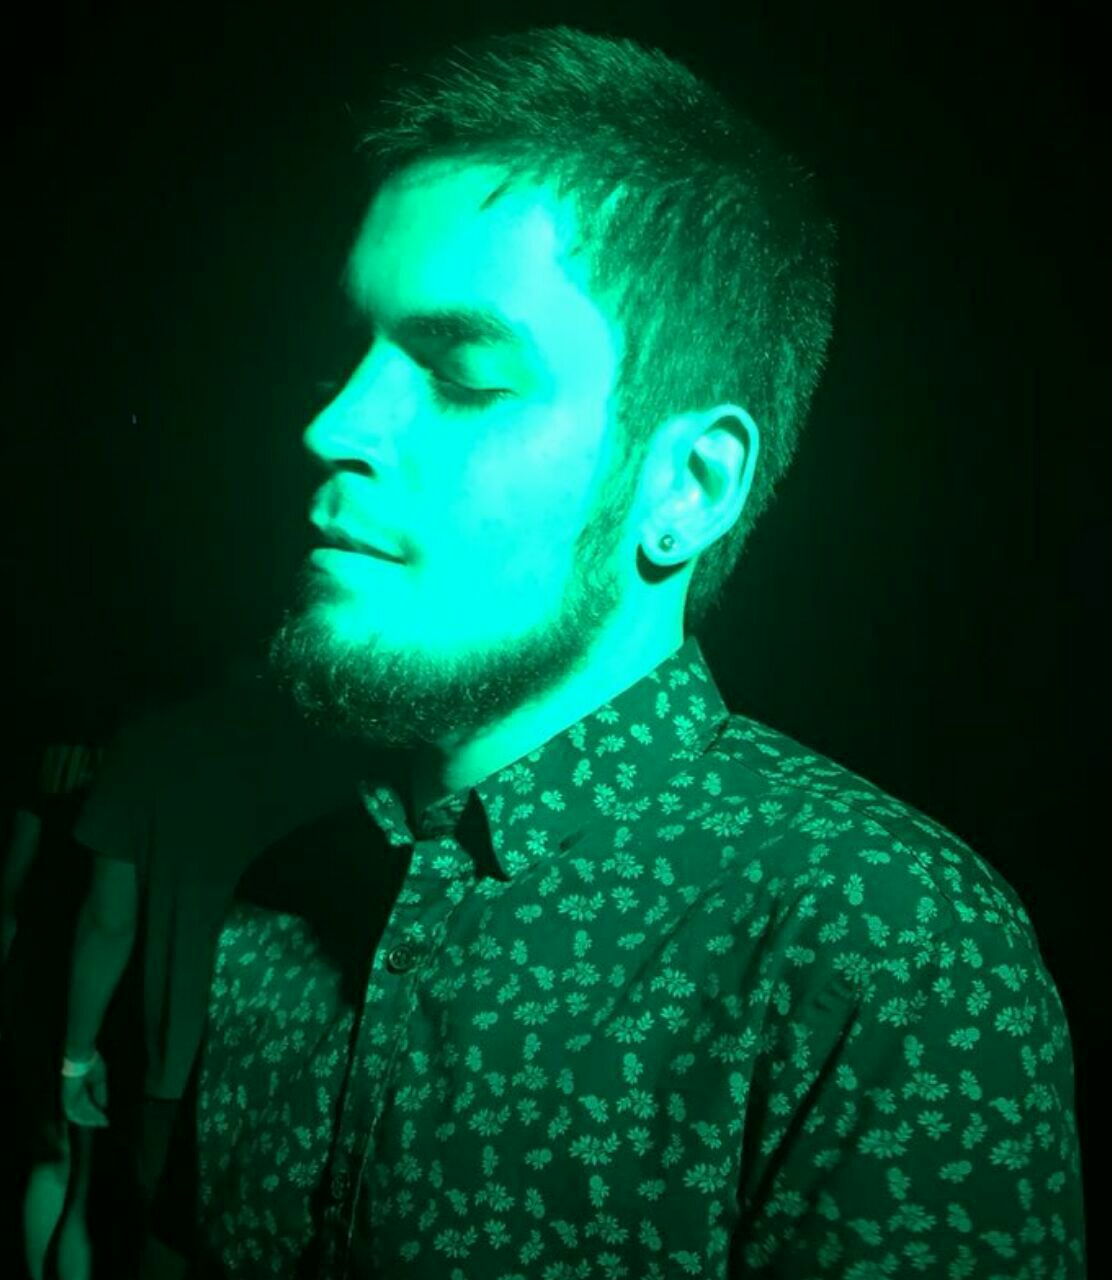
\includegraphics[width=\textwidth]{eu}
               };
           }]{};
\end{minipage} \hfill
\begin{minipage}{0.69\textwidth} \justifying
{\Large{\textbf{Olá!}} Eu sou o \textbf{Minho}.} 

\begin{itemize}
	\item[$\leadsto$] Bacharel em Eng. de Computação (UFC, 2019)
	\item[$\leadsto$] Mestrando em Eng. de Teleinformática (UFC, 2019--)
\end{itemize}

Sou um pesquisador com especialidade em \textbf{Aprendizagem de Máquina} e \textbf{Teoria do Controle}. \vskip0.25cm

\textbf{Contatos:} \vskip0.1cm
\begin{tabular}{c c c}
\begin{tikzpicture}
	\node (myman) {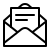
\includegraphics[width=13px]{email.png}};
	\node[below=-1mm of myman] {{\color{monokaiOrange!90!black} \bf minhotmog@gmail}};
\end{tikzpicture}
&
\begin{tikzpicture}
	\node (myman) {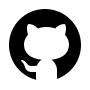
\includegraphics[width=13px]{github.png}};
	\node[below=-1mm of myman] {{\color{monokaiOrange!95!black} \bf @tiominho}};
\end{tikzpicture}
&
\begin{tikzpicture}
	\node (myman) {
\includegraphics[width=13px]{telegram.png}};
	\node[below=-1mm of myman] {{\color{monokaiOrange!90!black} \bf @katchau}};
\end{tikzpicture}
\end{tabular}
\end{minipage} 
\end{minipage} 

\vskip.3cm
\hrule
\vskip.3cm

Nessa palestra, iremos conversar sobre... \vskip0.1cm
\begin{varblock}[\textwidth]{} \centering
	{\bf \Huge Reinforcement Learning}
\end{varblock}


\end{frame}

%-------------------------------------------------------
\subsection{O que djabo é isso?}
%-------------------------------------------------------
\begin{frame}[t]{Apresentação}{} \vskip0.5cm

\begin{itemize}
	\item[$\leadsto$] Ramo da \textbf{I.A.} que lida com o controle autônomo de \textit{sistemas físicos reais}.
\end{itemize}

\begin{varblock}[\textwidth]{} \centering
\begin{tikzpicture}
	\node (1) [draw, rounded rectangle, fill=white] {\begin{tabular}{c}
													     Como programamos \\
													     máquinas para realizar \\
													     atividades que \\
													     exigem inteligência?
													  \end{tabular}};  
													  
	\node (2) [draw, right=1cm of 1, rounded rectangle, fill=white] {\begin{tabular}{c}
													     Como ensinar \\
													     máquinas a realizar \\
													     uma atividade \\
													     específica?
													  \end{tabular}};  

	\draw [->,thick] (1.north) to [out=15,in=165] (2.north);
	\draw [->,thick] (2.south) to [out=-165,in=-15] (1.south);
\end{tikzpicture}
\end{varblock}

\vskip0.3cm
\hrule
\vskip0.3cm

\begin{center}
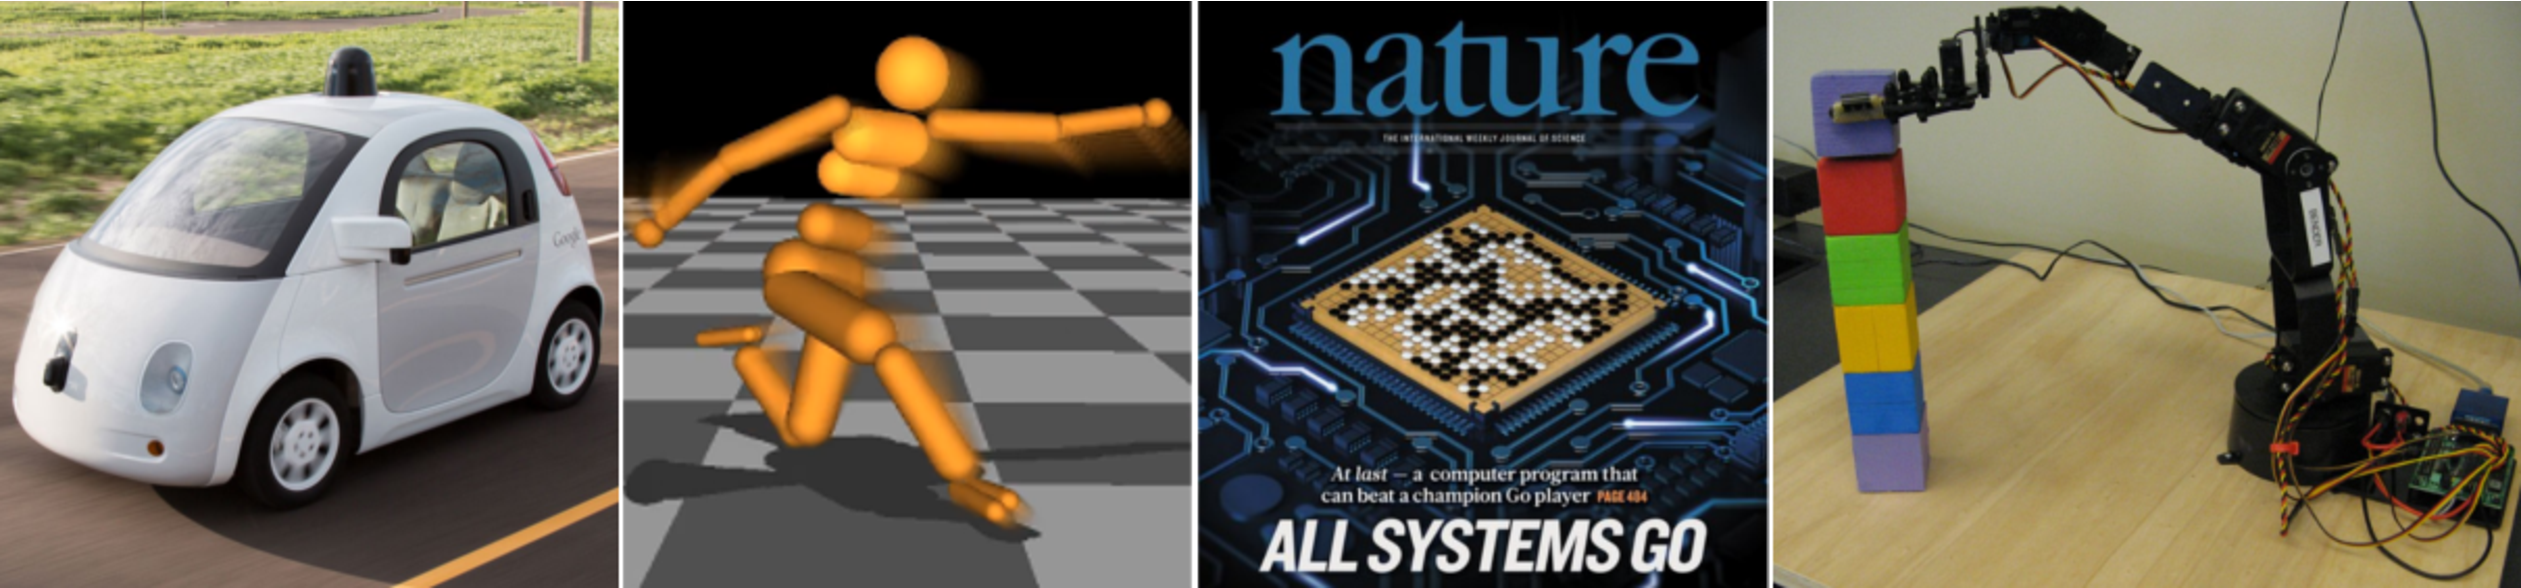
\includegraphics[width=0.9\textwidth]{examples}
\end{center}

\end{frame}

%-------------------------------------------------------
% SECTION - Agente Inteligente
%-------------------------------------------------------
\section{Agentes Inteligentes}
%-------------------------------------------------------
\subsection{Anatomia de um Agente}
%-------------------------------------------------------
\begin{frame}[t]{Agentes Inteligentes}{} \vskip0.3cm

{\large O elemento principal é o \textbf{Agente Inteligente}.} {\tiny (Também conhecido como ''Sistema Dinâmico'')}

\begin{varblock}[\textwidth]{} \centering
\begin{tikzpicture}
	\node (1) [draw, circle, fill=white] {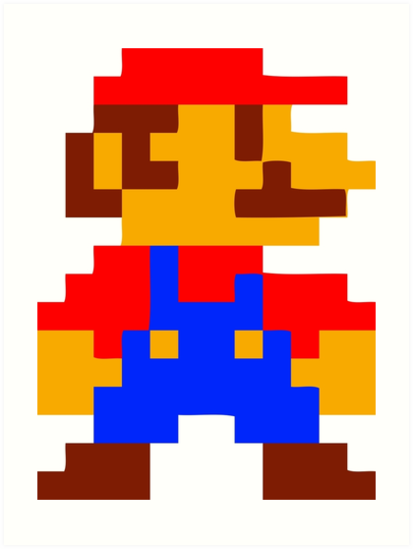
\includegraphics[width=30px]{mario}};  	
	
	\node (2) [draw, right=3.5cm of 1, rounded rectangle, minimum width=3.5cm, minimum height=2cm, 
					fill=white, fill overzoom image=marioStage]{};
													  
	\draw [->, thick] (1.north) |- node[text width=5cm,xshift=3cm,midway,above,align=center]{{\bf ATUADORES}\\{\small (O agente interage com o ambiente)}} ++(0,0.4) -| (2.north);
	\draw [->, thick] (2.south) |- node[text width=5cm,xshift=-3cm,midway,below,align=center]{{\bf SENSORES}\\{\small (O agente observa seu estado no ambiente)}} ++(0,-0.4) -| (1.south);
\end{tikzpicture}
\end{varblock}

\begin{itemize}
	\item[$\leadsto$] Está sempre inserido em um \textbf{Ambiente} que influencia um no outro.
	\item[$\leadsto$] Possui um conjunto de \textbf{ações} e \textbf{estados} possíveis.
	\item[$\leadsto$] Regidos por \textbf{leis bem definidas} \textit{(leis da física, regras de jogo, etc)}.
\end{itemize} \vskip0.4cm

\end{frame}

%-------------------------------------------------------
\subsection{Exemplos}
%-------------------------------------------------------
\begin{frame}[t]{Agentes Inteligentes}{} \vskip0.3cm

{\large \textbf{Exemplo:} Pêndulo Invertido} (ou ''\textit{Cartpole}'')

\begin{center}
	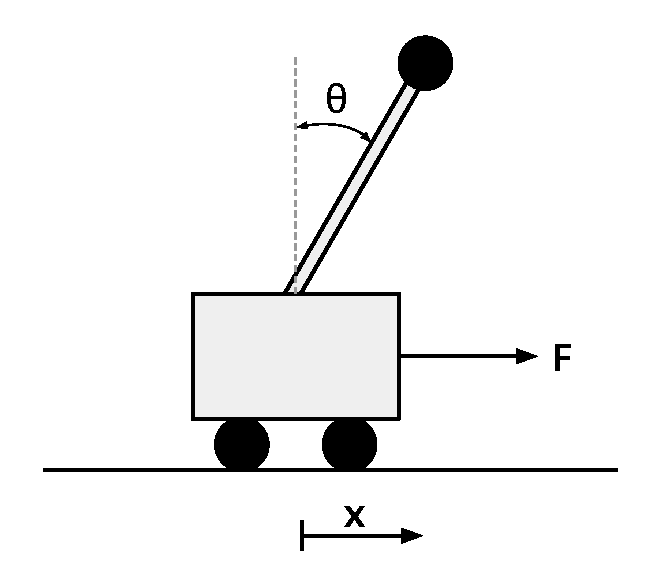
\includegraphics[width=5.5cm]{cartpole_crop}
\end{center} \vskip-0.6cm

{\Large \begin{equation*}
\begin{matrix}
{\color{monokaiOrange} \leadsto} \textbf{ Ações: } \begin{bmatrix} \Leftarrow, & \Rightarrow \end{bmatrix}
& & & &
{\color{monokaiOrange} \leadsto} \textbf{ Estados: } \begin{bmatrix} \bm{\theta}, & \bm{x} \end{bmatrix}
\end{matrix}
\end{equation*}}

\begin{flushright}
	\textbf{Spoiler:} vamos ver o Pêndulo\\ aprendendo a se controlar jajá
\end{flushright}

\end{frame}

%-------------------------------------------------------
% SECTION - Aprendizagem do Agente
%-------------------------------------------------------
\section{Aprendizagem do Agente}
%-------------------------------------------------------
\subsection{Controle por Planejamento}
%-------------------------------------------------------
\begin{frame}[t]{Aprendizagem do Agente}{} \vskip0.3cm

\begin{center}
	{\large O nosso Agente é {\color{monokaiBG} \textbf{ONISCIENTE}}.}
\end{center} \vskip0.2cm

{{\bf \color{monokaiOrange} CONTROLE POR PLANEJAMENTO}}
\begin{varblock}[\textwidth]{}
\begin{enumerate}
	\item Informamos ao Agente seu \textbf{estado de partida} e o seu \textbf{estado objetivo} \vskip0.2cm
	
	\item O Agente calcula uma \textbf{trajetória} $\leadsto$ (uma série de ações) \vskip0.2cm
	
	\item O Agente começa a aplicar sua \textbf{Lei de Controle} e recalcula a trajetória se houver algum desvio do que foi planejado \vskip0.2cm
\end{enumerate}
\end{varblock} \vskip0.3cm

\begin{minipage}{\textwidth} \centering
\begin{minipage}{.48\textwidth}
{\bf \color{retroGreen} Vantagens:}
\begin{itemize}
	\item Controle da melhor qualidade possível
	\item Algoritmos rápidos e implementáveis em chip
\end{itemize}
\end{minipage} \hfill
\begin{minipage}{.48\textwidth}
{\bf \color{retroRed} Desvantagens:}
\begin{itemize}
	\item Necessidade de \textbf{Modelos Dinâmicos}
	\item Altamente complexo para o programador
\end{itemize}
\end{minipage}
\end{minipage}

\vskip0.3cm
\textbf{Alguns algoritmos...}
\begin{itemize}
	\item[$\leadsto$] LQR, LQG, MPC, NMPC, iLQR, LoopShaping, DynamicProgramming, SMC, IPM, ...
\end{itemize}

\vfill
\begin{flushright}
	
\includegraphics[width=1.5cm]{pikachu}
\end{flushright} 

\end{frame}

%-------------------------------------------------------
\begin{frame}[t]{Aprendizagem do Agente}{} \vskip0.3cm

{\large \textbf{Modelos Dinâmicos} não são simples...}\\
{\tiny na verdade, essa é uma das maiores áreas de TODA a ciência}

\begin{center}
	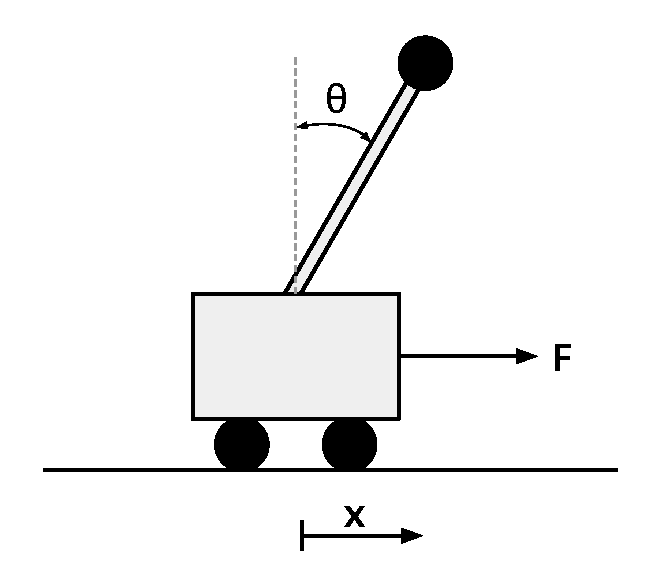
\includegraphics[width=5cm]{cartpole_crop}
\end{center} \vskip-0.6cm

{\small \begin{align*}
& {\color{monokaiOrange} \leadsto} \textbf{ Modelo: } \begin{bmatrix} \ddot{x} &=& \cfrac{2a}{2-m a cos^2(\theta)} \left( m l \theta^2 sin(\theta) - 0.5 m g cos(\theta) sin(\theta) + u - f_c(\dot{x}) + \cfrac{1}{2l} cos(\theta) d_{Mf} \dot{\theta} \right) \\
\ddot{\theta} &=& \cfrac{1}{2l-m l a cos^2(\theta)} \left( g sin(\theta) - m l a \dot{\theta} cos(\theta) + a cos(\theta)(u - f_{c}(\dot{x})) - \cfrac{d_{Mf} \dot{\theta}}{m l} \right) \end{bmatrix}
\\
& {\color{monokaiOrange} \leadsto} \textbf{ Ação->Estado: } x(t) = e^{At} x(t_0) + \int_{0}^{t} e^{A(t-\tau)} B u(\tau) d\tau
\end{align*}}

\end{frame}

%-------------------------------------------------------
\subsection{Controle por Recompensa}
%-------------------------------------------------------
\begin{frame}[t]{Aprendizagem do Agente}{} \vskip0.3cm

\begin{center}
	{\large O nosso Agente é {\color{monokaiBG} \textbf{MOTIVADO}}.}
\end{center} 

{{\bf \color{monokaiOrange} CONTROLE POR RECOMPENSA}}
\begin{varblock}[\textwidth]{}
\begin{enumerate}
	\item Criamos um \textbf{Sistema de Recompensas} para o Agente \vskip0.2cm
	
	\item O Agente verifica seu estado e... 
	\begin{itemize}
		\item \textit{(Exploração)} Tenta fazer uma ação que tenha \textbf{boa recompensa}, ou
		\item \textit{(Exploitação)} Faz qualquer ação \textbf{aleatória}
	\end{itemize}\vskip0.2cm
	
	\item Se a ação der recompensa, memoriza a relação (Estado $\rightarrow$ Ação) como boa. \vskip0.2cm
	
	\item Repete o processo até o Agente aprender todas as relações, ou você perder a paciência. \vskip0.2cm
\end{enumerate}
\end{varblock} \vskip0.2cm

\begin{minipage}{\textwidth} \centering
\begin{minipage}{.48\textwidth}
{\bf \color{retroGreen} Vantagens:}
\begin{itemize}
	\item Não precisa de modelos, só de treino
	\item Simula a forma como seres humanos aprendem
\end{itemize}
\end{minipage} \hfill
\begin{minipage}{.48\textwidth}
{\bf \color{retroRed} Desvantagens:}
\begin{itemize}
	\item Treinamento é demorado e caro
	\item O resultado dificilmente será perfeito
\end{itemize}
\end{minipage}
\end{minipage}

\vskip0.2cm
\textbf{Alguns algoritmos...}
\begin{itemize}
	\item[$\leadsto$] Q-Learning, TD, SARSA, ADP, E2ERL, Policy Gradients, DeepQN, ...
\end{itemize}

\end{frame}

%-------------------------------------------------------
\begin{frame}[t]{Aprendizagem do Agente}{} \vskip0.3cm

{\large {\bf \color{monokaiOrange} Redes Neurais:} codificação biológica de {\it (Atuadores, Sensores)}}

\vfill

\begin{center}
	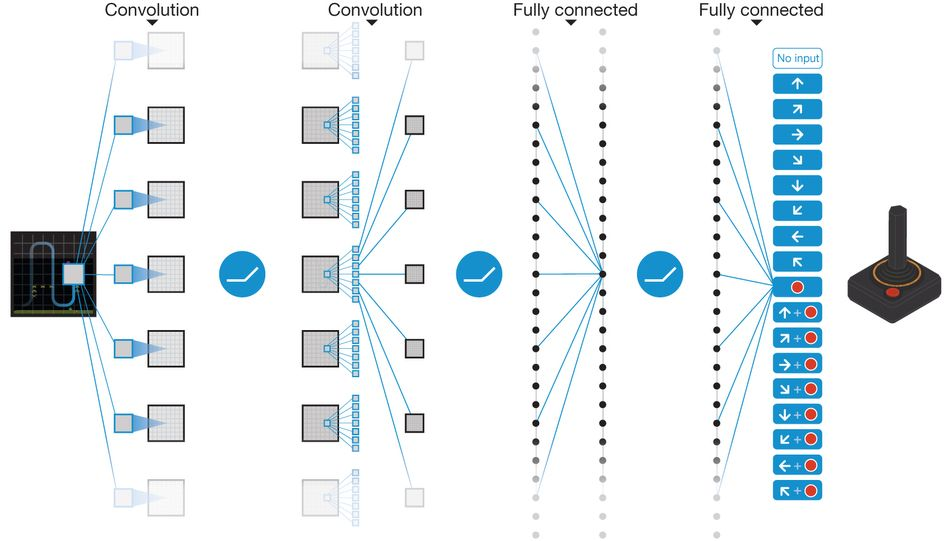
\includegraphics[width=0.85\textwidth]{natureDQN}
\end{center}

\end{frame}

%-------------------------------------------------------
% SECTION - ! Showcase !
%-------------------------------------------------------
\section{! Showcase !}
%-------------------------------------------------------

%-------------------------------------------------------
%-------------------------------------------------------
%-- End Page
{\1
\begin{frame}[plain,noframenumbering]
  \center \Huge \textbf{\color{monokaiOrange} Muito obrigado!}       
  
  
\includegraphics[scale=0.4]{corgi.jpg}
  
  {\color{monokaiOrange} Perguntas?}       
\end{frame}

%-------------------------------------------------------
\end{document}


%%---------------------Rascunho--------------------------
%\section{Titulo}
%\subsection{Subtitulo}
%%---------------------Rascunho--------------------------
%\begin{frame}{Titulo}{Subtitulo}
%
%\begin{block}{title}
% Say somethings \alert{new} 
%\end{block}
%
%\begin{itemize}
% \item TikZ\footnote{TikZ is a package for creating beautiful graphics. Have a look at these \chref{http://www.texample.net/tikz/examples/}{online examples} or the \chref{http://tug.ctan.org/tex-archive/graphics/pgf/base/doc/generic/pgf/pgfmanual.pdf}{pgf user manual}.}
%\end{itemize}
%
%\end{frame}
%%---------------------Rascunho--------------------------

%%%%%%%%%%%%%%%%%%%%%%%%%%%%%%%%%%%
%% Drafts:
%%%%%%%%%%%%%%%%%%%%%%%%%%%%%%%%%%%
%%%%% Figure:
% \begin{figure}[ht]
%   \centering
%   \includegraphics[trim={0cm 0cm 0cm 0cm},clip,scale=1]{nameFigure}
%   \caption{caption of the figure.}
%   \label{fig:nameFigure}
% \end{figure} \vskip0.25cm
%
%%%%% Equation:
% \begin{equation*} \label{eq:nameequation*}
% \begin{split}
%  X = 1 + 1
% \end{split}
% \end{equation*} \vskip0.25cm
%
%%%% Table:
% \begin{table}[hp]
%   \centering
%   \begin{tabular}{l | c c }
%   Principal & Coluna1 & Coluna2 \\
%   \hline 
%   ABC & 1 & 2 \\
%   DFG & 3 & 4 \\
%   HIJ & 5 & 6 \\
%   \end{tabular} 
%   \caption{caption of the table.}
%   \label{table:nameTable} 
% \end{table} \vskip0.25cm
